\documentclass[border=10pt]{standalone}
\usepackage{tikz}
\begin{document}
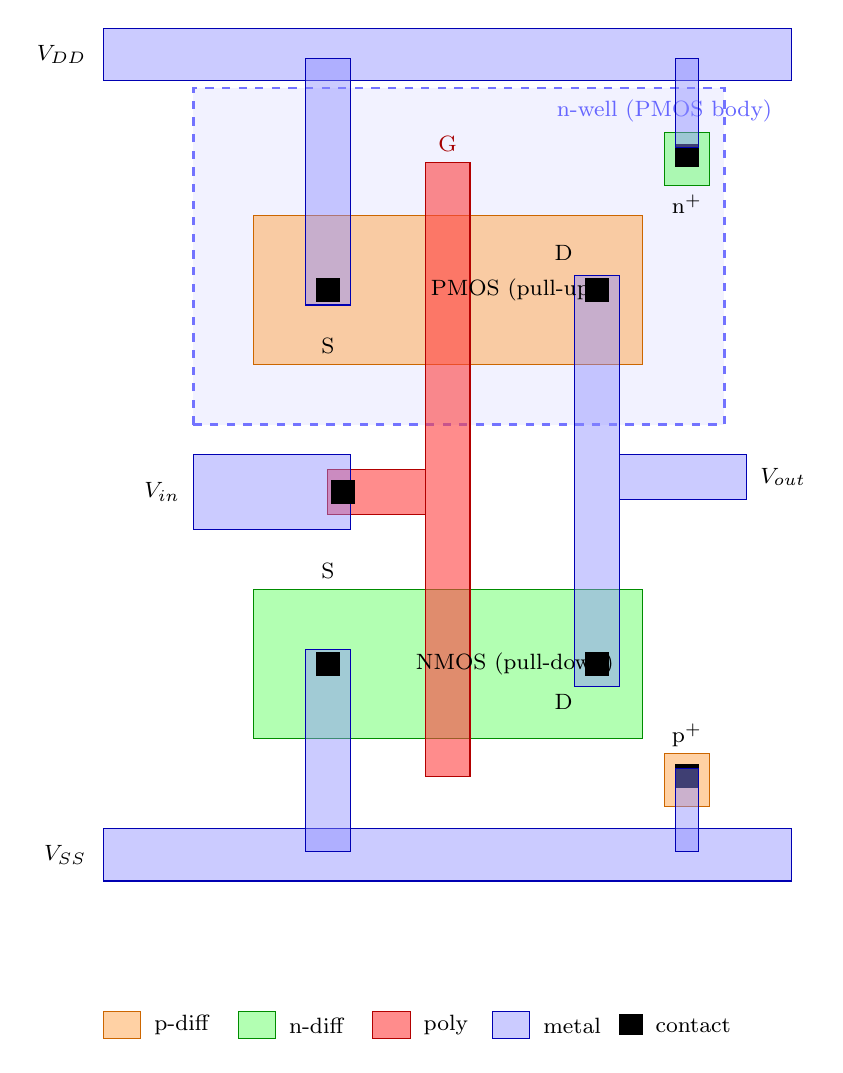
\begin{tikzpicture}[scale=0.95,
  nwell/.style ={draw=blue!55, dashed, line width=1pt, fill=blue!5},
  pdiff/.style ={draw=orange!80!black, fill=orange!65, fill opacity=0.55},
  ndiff/.style ={draw=green!55!black, fill=green!60, fill opacity=0.5},
  poly/.style  ={draw=red!70!black,  fill=red!75,  fill opacity=0.6},
  metal/.style ={draw=blue!70!black, fill=blue!45, fill opacity=0.45},
  cont/.style  ={draw=black, fill=black},
  lbl/.style   ={font=\footnotesize}]

  % ---------------- power rails ----------------
  \fill[metal] (0.4,11.0) rectangle (9.6,11.7);  \node[lbl,left] at (0.3,11.35){$V_{DD}$};
  \fill[metal] (0.4,0.3)  rectangle (9.6,1.0);    \node[lbl,left] at (0.3,0.65){$V_{SS}$};

  % ---------------- n-well around PMOS ----------------
  \fill[nwell] (1.6,6.4) rectangle (8.7,10.9);
  \node[lbl,blue!60] at (7.9,10.6){n-well (PMOS body)};

  % ---------------- active areas ----------------
  \fill[pdiff] (2.4,7.2) rectangle (7.6,9.2);     % PMOS p-diffusion
  \fill[ndiff] (2.4,2.2) rectangle (7.6,4.2);     % NMOS n-diffusion

  % ---------------- polysilicon gate (vertical, shared) ----------------
  \fill[poly] (4.7,1.7) rectangle (5.3,9.9);
  \node[lbl,red!65!black] at (5.0,10.15){G};
  % gate input tab to the left + Vin contact
  \fill[poly]  (4.7,5.2) rectangle (3.4,5.8);
  \fill[metal] (1.6,5.0) rectangle (3.7,6.0);
  \fill[cont]  (3.45,5.35) rectangle (3.75,5.65);
  \node[lbl,left] at (1.55,5.5){$V_{in}$};

  % ---------------- PMOS source -> VDD (left of gate) ----------------
  \fill[metal] (3.1,8.0) rectangle (3.7,11.3);
  \fill[cont]  (3.25,8.05) rectangle (3.55,8.35);
  \node[lbl] at (3.4,7.45){S};

  % ---------------- NMOS source -> VSS (left of gate) ----------------
  \fill[metal] (3.1,0.7) rectangle (3.7,3.4);
  \fill[cont]  (3.25,3.05) rectangle (3.55,3.35);
  \node[lbl] at (3.4,4.45){S};

  % ---------------- Vout : vertical metal joins both drains (right of gate) ----
  \fill[metal] (6.7,2.9) rectangle (7.3,8.4);
  \fill[cont]  (6.85,8.05) rectangle (7.15,8.35);   % PMOS drain
  \fill[cont]  (6.85,3.05) rectangle (7.15,3.35);   % NMOS drain
  \node[lbl] at (6.55,8.7){D}; \node[lbl] at (6.55,2.7){D};
  \fill[metal] (7.3,5.4) rectangle (9.0,6.0);
  \node[lbl,right] at (9.05,5.7){$V_{out}$};

  % ---------------- well tap (n+ -> VDD) & substrate tap (p+ -> VSS) ----------------
  \fill[ndiff] (7.9,9.6) rectangle (8.5,10.3);
  \fill[cont]  (8.05,9.85) rectangle (8.35,10.15);
  \fill[metal] (8.05,10.1) rectangle (8.35,11.3);
  \node[lbl] at (8.2,9.35){n$^{+}$};
  \fill[pdiff] (7.9,1.3) rectangle (8.5,2.0);
  \fill[cont]  (8.05,1.55) rectangle (8.35,1.85);
  \fill[metal] (8.05,0.7) rectangle (8.35,1.8);
  \node[lbl] at (8.2,2.25){p$^{+}$};

  % ---------------- device labels ----------------
  \node[lbl] at (5.9,8.2){PMOS (pull-up)};
  \node[lbl] at (5.9,3.2){NMOS (pull-down)};

  % ---------------- legend ----------------
  \begin{scope}[shift={(0,-2.3)}]
    \fill[pdiff](0.4,0.5) rectangle(0.9,0.85); \node[lbl,right] at(0.95,0.67){p-diff};
    \fill[ndiff](2.2,0.5) rectangle(2.7,0.85); \node[lbl,right] at(2.75,0.67){n-diff};
    \fill[poly] (4.0,0.5) rectangle(4.5,0.85); \node[lbl,right] at(4.55,0.67){poly};
    \fill[metal](5.6,0.5) rectangle(6.1,0.85); \node[lbl,right] at(6.15,0.67){metal};
    \fill[cont] (7.3,0.55) rectangle(7.6,0.82); \node[lbl,right] at(7.65,0.67){contact};
  \end{scope}
\end{tikzpicture}
\end{document}
